\documentclass[main.tex]{subfiles}
\usepackage{tikz}
\usetikzlibrary{arrows.meta, positioning}
\usepackage{graphicx}


\begin{document}
\section{Estimation}
\begin{frame}[fragile]
    \frametitle{Introductory example}
\begin{block}{Delays dataset}
   \begin{itemize}
    \item<+-> Download the file "delays.csv" and open it in PowerBI. Use the "Table" pane and find the maximum and minimum values of the
    third column. 
    \item<+-> Negative delays are not of interest for us, nor delays higher than 3h, that are outliers. Create a new table with the command:
    {\footnotesize 
    \begin{verbatim}
pos_delays = 
FILTER(delays,delays[Column3]>=0 && delays[Column3]<=10000)
    \end{verbatim}}
    \item<+-> Using an "R" visual, plot the histogram of the delays in the new table with the option \texttt{freq=FALSE} to display probabilities.
    Since PowerBI removes duplicate values, be sure to include all columns in the plot.
\end{itemize}
\end{block}
\end{frame}
\begin{frame}
    \frametitle{Introductory example}
\begin{block}{Modeling the delays}
   \begin{itemize}
    \item<+-> Compute the inverse of the average of the delays.
    \item<+-> Use an R script to generate an exponentially distributed sample of size 100000 (use the \texttt{rexp} command) with rate the above value.
    \item<+-> Compare the histogram of the values with the one coming from the delays dataset. 
    \item<+-> Do you think that assuming an exponential distribution for the delays is reasonable ?
   \end{itemize} 
\end{block}
\end{frame}
\begin{frame}
    \frametitle{Estimation}
\begin{block}{Population vs sample}
    \begin{itemize}
        \item<+-> In the previous example, the dataset of delays is a sample, i.e. a set of \textbf{observations}.
        \item<+-> The associated population is an hypothetical measure space describing all possible delays.
    \end{itemize}
\end{block}
\end{frame}

\begin{frame}

\begin{block}{Illustration: Population vs sample}
    \begin{center}
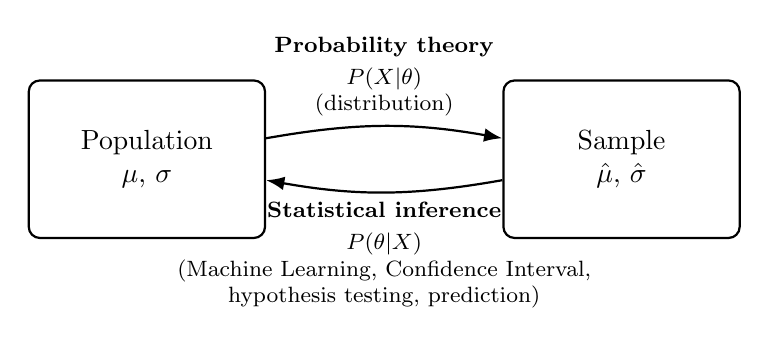
\begin{tikzpicture}[
  box/.style={draw, thick, rounded corners, minimum width=3cm, minimum height=2cm, align=center},
  arrow/.style={-Latex, thick},
  note/.style={align=center, font=\footnotesize}
]

% Population box
\node[box] (pop) {Population\\ $\mu$, $\sigma$};

% Sample box
\node[box, right=3cm of pop] (samp) {Sample\\ $\hat{\mu}$, $\hat{\sigma}$};

% Probability theory arrow (Population → Sample)
\draw[arrow, bend left=10] (pop) to node[above, note]{\textbf{Probability theory}\\[2pt] $P(X|\theta)$\\(distribution)} (samp);

% Statistical inference arrow (Sample → Population)
\draw[arrow, bend left=10] (samp) to node[below, note]{\textbf{Statistical inference}\\[2pt] $P(\theta|X)$\\(Machine Learning, Confidence Interval, \\hypothesis testing, prediction)} (pop);


\end{tikzpicture}
\end{center}
\vspace{0.5em}
\begin{itemize}
  \item \textbf{Goal:} Model and quantify uncertainty using data.
  \item Descriptive statistics:  summarize the sample

  \item Probability theory: from population assumptions $\rightarrow$ data behavior.
  \item Statistical inference: from observed data $\rightarrow$ population insights.
\end{itemize}
\end{block}
\end{frame}


\begin{frame}
    \frametitle{Estimation}
\begin{block}{Statistical model}
   \begin{itemize}
    \item<+-> An statistical model is a triple $\left( \Omega, \mathcal{T}, \mathcal{P} \right)$ where $\Omega$ is a sample space,
    $\mathcal{T}$ a $\sigma$-algebra on $\Omega$ and $\mathcal{P}$ a set of probabilities on $\mathcal{T}.$
    \item<+-> The population associated with the studied sample hopefully belongs to $\mathcal{P}$\dots
   \end{itemize} 
\end{block}
\begin{block}{Kinds of models}
\begin{itemize}
    \item<+-> If $\mathcal{P}$ can be fully described by a finite number of parameters, the model is said to be \textbf{parametric}. As an example, 
    the set of exponential distributions is parameterized by the rate.
    \item<+-> If $\mathcal{P}$ can be partly described by a finite number of parameters, the model is said to be \textbf{semi-parametric}.
    \item<+-> In all the other cases, the model is \textbf{non-parametric}.
    \item<+-> In the course, only parametric models are considered. 
\end{itemize}    
\end{block}
 
\end{frame}
\begin{frame}
    \frametitle{Estimation}
\begin{block}{Estimation}
    \begin{itemize}
        \item<+-> Let the population has probability measure $P \in \mathcal{P}$.
        \item<+-> Assume that independent random variables $X_1,\dots, X_n$ have the identical distribution $P$.
        \item<+-> Estimation is the process of finding $P$ using the sample $X_1,\dots,X_n$.
        \item<+-> When the model is parametric, an estimator of a parameter is a 
        random variable $Y=f\left( X_1,\dots ,X_n \right)$ where $f$ does not depend on the parameter.
    \end{itemize}
 \end{block}
\end{frame}
\begin{frame}
    \frametitle{Bias and consistency}
\begin{itemize}
\item<+-> Assuming $\theta$ is the true value of the parameter to be estimated,
and $f\left( X_1, \dots, X_n \right)$ is the estimator, the bias is:
\begin{equation}
    E\left[ f\left( X_1,\dots X_n \right) \right] - \theta.
\end{equation}
\item<+-> If the bias vanishes, the estimator is said to be unbiased.
\item<+-> The mean square error of the estimator is:
\begin{equation}
    MSE_f(X_1,\dots, X_n)= E\left[ \left( f(X_1, \dots X_n) - \theta \right)^2 \right]
\end{equation}
\item<+-> An estimator is said to be consistent if, for any $\epsilon > 0$:
\begin{equation}
    \lim_{n \to +\infty}P\left( \lvert f(X_1,\dots,X_n) - \theta\rvert > \epsilon \right) = 0.
\end{equation} 
\end{itemize}
\end{frame}
\begin{frame}
    \frametitle{Consistency}
    \begin{block}{Bienaymé–Chebyshev inequality}
        Let $X$ be a random variable. Then, for any
        $\epsilon > 0$:
        \begin{equation}
            \label{eq:Chebyshev}
            P\left( \lvert X- E\left[ X \right] \rvert \geq \epsilon \right) \leq \frac{V(X)}{\epsilon^2}.
        \end{equation}
    \end{block}
    \begin{block}{MSE and consistency}
        \begin{itemize}
            \item<+-> The next two properties are consequences of \ref{eq:Chebyshev}.
            \item<+-> If an estimator $f\left( X_1, \dots, X_n \right)$ is unbiased, then it is consistent
    if its variance goes to 0 as $n$ goes to $+\infty$.
            \item<+-> For any estimator, if $\lim_{n \to +\infty} MSE_f\left( X_1,\dots,X_n \right) = 0,$ then
            the estimator is consistent.
            \item<+-> From now, an estimator of $\theta$ will be denoted $\hat{\theta},$ letting the sample be implicit.
        \end{itemize}
    \end{block}
\end{frame}
\begin{frame}
    \frametitle{Method of moments}
\begin{itemize}
    \item<+-> This procedure is one of the most common in practice.
    \item<+-> If the parameter $\theta$ to be estimated is a moment $E\left[ X^k \right]$ of the population probability measure, then
    the sample mean:
    \begin{equation}
        \hat{\theta} = \frac{1}{n} \sum_{i=1}^n X_i^k
    \end{equation}
    is an unbiased and consistent estimator.
    \item<+-> If $g$ is a continuous function, $g\left(\hat{\theta}\right)$ is generally not an unbiased estimator of $g\left( \theta \right)$, it is, 
    however, consistent.
\end{itemize}
\end{frame}

\begin{frame}
\begin{block}{Exercise with R: Understand estimators\\}
Objectives:
\begin{itemize}
  \item Understand the concept of estimation in statistics.
  \item Differentiate between sample and population parameters.
  \item Use R to estimate the population mean and variance.
  \item Explore the effect of sample size on estimation accuracy.
\end{itemize}
\end{block}
\end{frame}


\begin{frame}
\begin{block}{Part 1: Generating Data\\}
\textbf{Task (5 min):} Simulate a population using $$\texttt{population <- rnorm(100000, mean = 50, sd = 10)}$$
to create a dataset in PowerBI.
% \begin{lstlistings}[language=R]
% set.seed(123)
% population <- rnorm(100000, mean = 50, sd = 10)
% hist(population, main = "Population Distribution", col = "skyblue")
% \end{lstlistings}
\textbf{Answer questions:}
\begin{itemize}
  \item<+-> Plot the histogram of the population.
  \item<+-> What probability distribution does the population follow? Can you relate the population parameters ($\mu$, $\sigma^2$) to moments ?
  \item<+-> Do we usually know these values in practice?
\end{itemize}
\end{block}
\end{frame}

\begin{frame}
\begin{block}{Part 2: Sample Estimation\\}
\textbf{Task (10 min):} Draw samples of different sizes of 10, 50, and 200, and compute sample mean and variance.
 $$\texttt{sample10 <- sample(population, 10);}$$
\textbf{Answer questions:}
\begin{itemize}
  \item Do larger samples give more stable estimates of the mean?
  \item How close are the sample means to the true mean (50)?
  \item Does sample variance approximate the population variance well?
\end{itemize}
\end{block}
\end{frame}


\begin{frame}
\begin{block}{\\Part 3: Sampling Distribution\\}
\textbf{Task (10 min):} Examine variability in estimates using simulation:
\begin{enumerate}
\small
  \item Set the sample size $n=30$
  \item Set the number of simulations $\text{nsim} = 1000$
  \item Draw 1000 random samples (of size 30) from the population and record each sample mean.
  \item Plot a histogram of the sample means.
    \item Compute and report the mean and standard deviation of the sample means.
\end{enumerate}
% \begin{lstlistings}[language=R]
% n <- 30
% nsim <- 1000
% means <- replicate(nsim, mean(sample(population, n)))
% hist(means, main="Sampling Distribution of the Mean", col="lightgreen")
% mean(means); sd(means)
% \end{lstlistings}
\textbf{Answer questions:}
\begin{itemize}
\small
  \item What is the average of the sample means?
  \item Does it approximate the true mean (unbiasedness)?
  \item What happens to the spread (or variability) of the means if $n$ increases?
  \item Can you relate this to the Central Limit Theorem?
\end{itemize}
\end{block}
\end{frame}


\begin{frame}
\begin{block}{Summary and Reflection\\}
\textbf{Key Takeaways:}
\begin{itemize}
  \item Sample estimates approximate unknown population parameters.
  \item Larger samples yield more precise estimates.
  \item Sampling distributions provide a basis for inference.
  % \item Confidence intervals quantify estimation uncertainty.
\end{itemize}

\textbf{Reflection:}
\begin{itemize}
  \item What assumptions underlie these estimations?
  \item How would results differ for non-normal populations?
  \item How might bias arise in practical data collection?
\end{itemize}
\end{block}
\end{frame}
\begin{frame}[fragile]
    \frametitle{Exponential distribution}
    \begin{itemize}
        \item<+-> This exercise is an illustration of the method of moments.
        \item<+-> Using PowerBI and R, generate a sample from an exponential distribution with rate 2:
\begin{verbatim}
sim_exp <- data.frame(n=1:10000,x=rexp(10000,rate=2))
\end{verbatim}
        \item<+-> Compare the average of the dataset with the inverse of the rate. 
    \end{itemize}
\end{frame}
\end{document}
